\section{ACTIVIDAD 02 Creación de un Data Source View}

Si bien es cierto hemos creado una conexión hacia Adventure Works DW, solo trabajaremos con algunas tablas. 			Seleccionamos las tablas DimDate,DimProduct y FactInternetSales:
	\begin{center}
	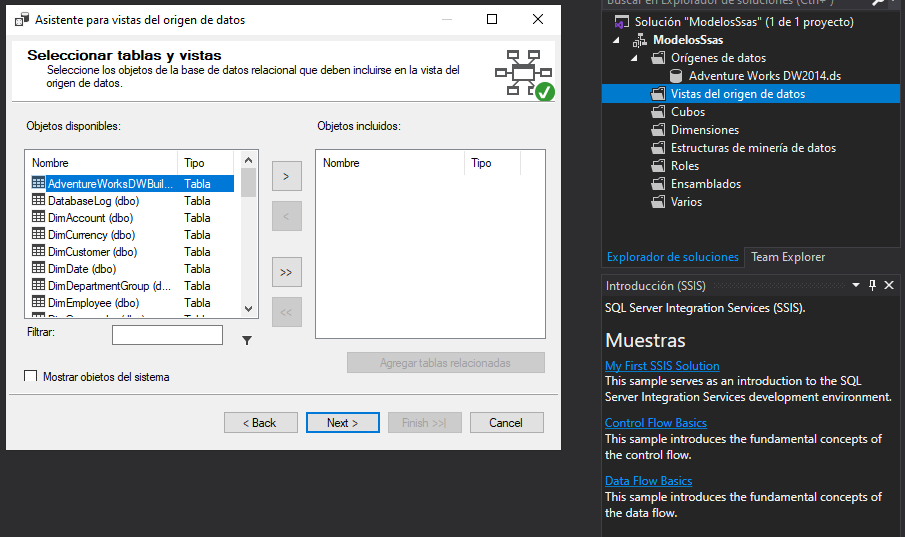
\includegraphics[width=\columnwidth]{images/task1/9}
    \end{center}	
    
Colocamos un nombre el Data Source View creado y click en Finish:
	\begin{center}
	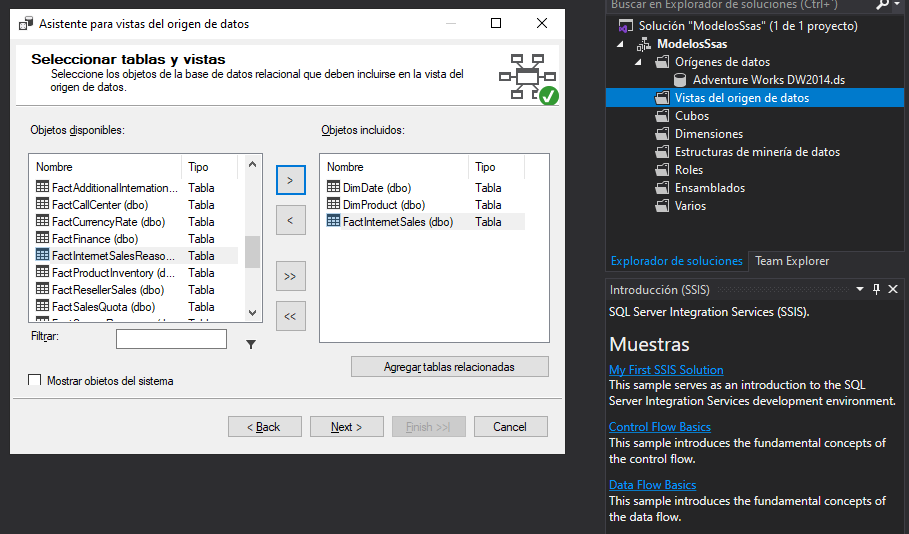
\includegraphics[width=\columnwidth]{images/task1/10}
    \end{center}	
    
	\begin{center}
	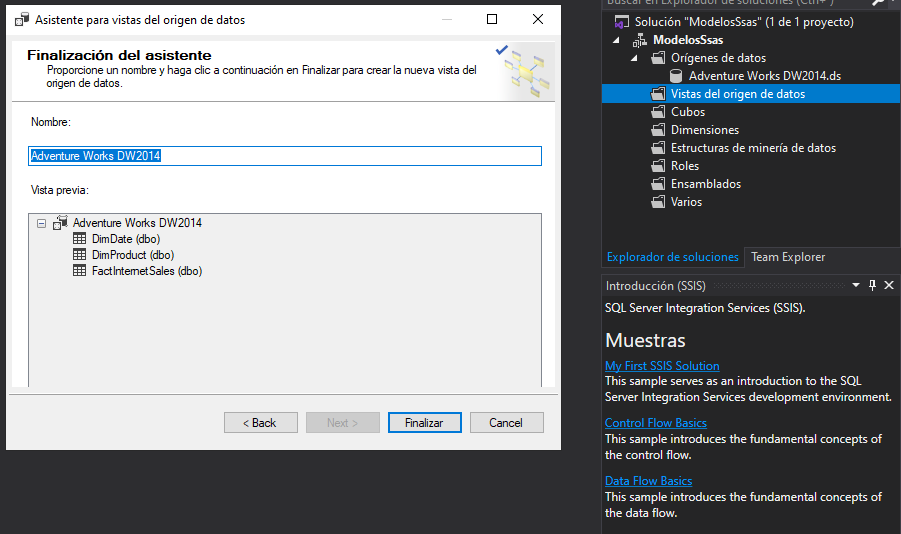
\includegraphics[width=\columnwidth]{images/task1/11}
    \end{center}	
    
Si todo va bien visualizaremos las tablas seleccionadas en el Data Source View:
	\begin{center}
	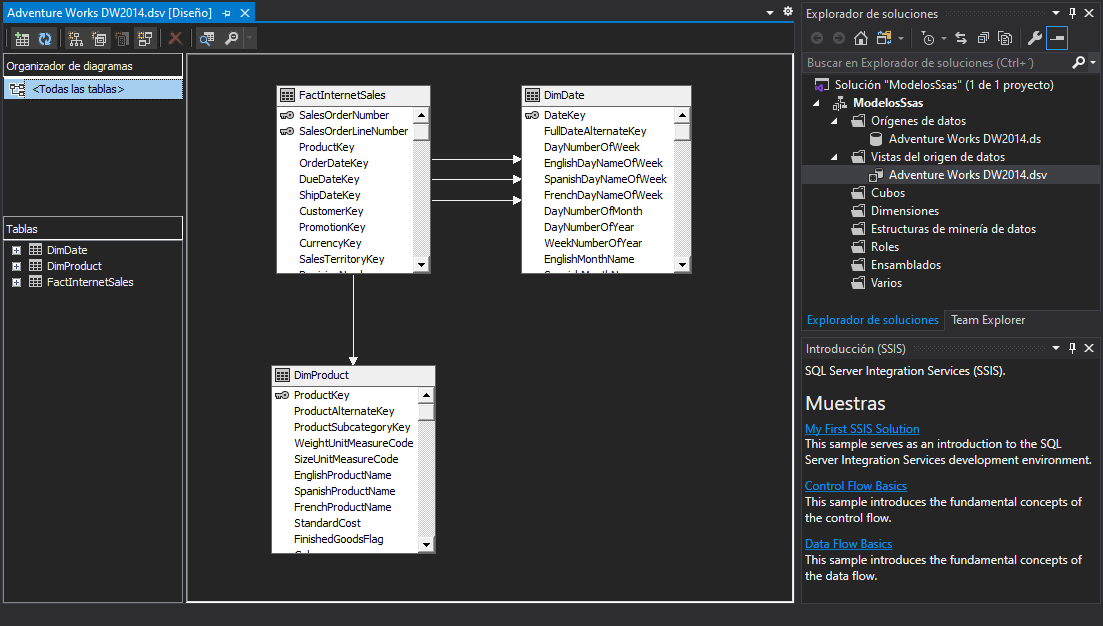
\includegraphics[width=\columnwidth]{images/task1/12}
	\end{center}	